%
% Modified by Megan Patnott
% Last Change: Jan 18, 2013
%
%%%%%%%%%%%%%%%%%%%%%%%%%%%%%%%%%%%%%%%%%%%%%%%%%%%%%%%%%%%%%%%%%%%%%%%%
%
% Modified by Bryce Frentz
% Last Change: 2018
%
%%%%%%%%%%%%%%%%%%%%%%%%%%%%%%%%%%%%%%%%%%%%%%%%%%%%%%%%%%%%%%%%%%%%%%%%
%
% Sample Notre Dame Thesis/Dissertation
% Using Donald Peterson's ndthesis classfile
%
% Written by Jeff Squyres and Don Peterson
%
% Provided by the Information Technology Committee of
%   the Graduate Student Union
%   http://www.gsu.nd.edu/
%
% Nothing in this document is serious except the format.  :-)
%
% If you have any suggestions, comments, questions, please send e-mail
% to: ndthesis@gsu.nd.edu
%
%%%%%%%%%%%%%%%%%%%%%%%%%%%%%%%%%%%%%%%%%%%%%%%%%%%%%%%%%%%%%%%%%%%%%%%%

%
% Chapter 3
%

\chapter{Cross section data Reduction and analysis}
\label{chap: data}

\section{Introduction}

In aggregate, the data taken at both the CASPAR and NSL experiments consists of $\gamma$-ray energy data from the $^{14}$N$\left( p,\gamma \right) ^{15}$O reaction, observed with a single, 130\% HPGe detector placed at $55^{\degree}$ relative to the beam direction. These data were collected for reactions over the combined proton energy range of 270 - 1200 keV. The primary interest of these experiments was monitoring the R/DC$\rightarrow$GS transition and the R/DC$\rightarrow$6.79 MeV + 6.79 MeV$\rightarrow$GS transition sequence. As such, the energies of the concerned photons ranged in energy from $\sim$600 keV up to $\sim$8500 keV. This chapter details the processes by which this data is gathered and turned into an experimental cross section.

\section{Angular corrections}
\label{sec: angularCorrections}

The angular distribution of a cross section, $W$, can be described by

\begin{equation}
W_{\text{exp}} = a_{0} \left(1 + \sum_{i = 1}^{n} a_{i} Q_{i} P_{i} ( \cos (\theta) )    \right)
\end{equation}

\noindent where $a_{i}$ are the angular distribution coefficients, $Q_{i}$ are correction factors due to the finite size of a given detector, and the $P_{i} ( \cos (\theta) )$ are the Legendre polynomials of order $i$. For the conditions of this work, odd numbered terms as well as those of order higher than 2 give negligible contribution to the angular distribution. Therefore, the resulting angular distribution of this reaction is of the form

\begin{equation}
W_{\text{exp}} = a_{0} + a_{2} Q_{2} P_{2} ( \cos (\theta) ).
\end{equation}

Experimentally, to address any effects arising from an angular distribution of this form, the detector was placed at $55^{\degree}$. This is the zero of the 2nd order Legendre polynomial, thereby minimizing any effects on the cross section arising from the detector's angle. Simultaneously, this means that no correction of the data is necessary.


\section{Energy calibration}
\label{sec: energy calibration}

It is important to establish the true relationship between $\gamma$-rays of different energies incident in a detector and the signal they produce during data acquisition. This connection is determined by calibrating the system with $\gamma$-rays of well-known energy from room background, given radioactive sources, like $^{137}$Cs or $^{60}$Co, and well-studied nuclear reactions, like $^{27}$Al($p, \gamma$)$^{28}$Si. The reactions are also used in calibration because no natural sources of radioactivity provide $\gamma$'s with energy higher than 3.6 MeV, whereas the $^{27}$Al($p, \gamma$)$^{28}$Si reaction provides $\gamma$ ray energies up to 10.7 MeV, ensuring that the detector is well calibrated over the entire energy range for $\gamma$'s that will be seen in the $^{14}$N$\left( p,\gamma \right) ^{15}$O reaction. The exact relationship between the the channel number in the acquisition system analog-to-digital converter (ADC) and the incident photon energy, $E_{\gamma}$, is characterized by the standard linear relationship

\begin{equation}
E_{\gamma} = m \times \text{Channel} + b
\end{equation}

\noindent where $m$ is simply the slope and $b$ the offset of the fit. For a HPGe detector, a linear relationship is sufficient and appropriate to describe the ADC response. However, this process was redone for every phase of the experiment because slightly different gains applied to the ADC's and signal amplifiers provide a different relationship in the electronics. Therefore, despite using the same detector, each phase of the experiment required its own energy calibration, an example of which is shown in Fig.\ \


\begin{figure}
\centering
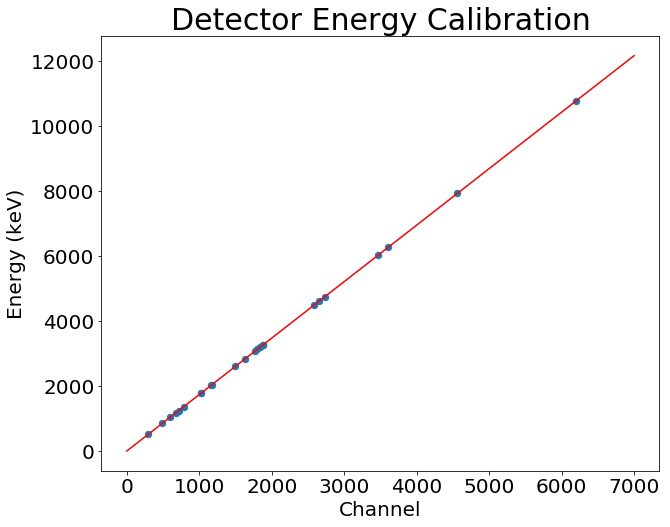
\includegraphics[width=0.8\linewidth]{figures/detEnergyCalibration.png}
\label{fig: energyCalibration}
\caption{Energy calibration curve for the HPGe detector taken at CASPAR. The calibration incorporated natural background, radioactive sources, and the products from the $^{27}$Al($p, \gamma$)$^{28}$Si reaction. }
\end{figure}




\section{Efficiency}
\label{sec: efficiency}

Efficiency is a term that can, in different contexts, have many different meanings. However, in experimental physics it is known to be the ratio for the response of an instrument to the actual physical quantity for which it is employed to measure. In these cases, it is the ratio between the photons recorded and those emitted in a given event. For this experiment, both the total efficiency, $\eta^{tot}$, and the full-energy peak (FEP) efficiency, $\eta^{fep}$, were required. The total efficiency is the probability that the $\gamma$ ray enters and deposits any amount of energy within the detector, while, on the other hand, the FEP efficiency is the probability that the full energy of an emitted $\gamma$ ray will be deposited within the detector. As both efficiency types are dependent on the physical geometry of the system, they are determined for each experimental setup in turn. 

\subsection{Total efficiency}

The total efficiency of a detector / source geometry is the probability that a given photon from the source will enter and deposit any amount of energy within the detector. For extremely simple geometries, the total efficiency can be calculated following the approach laid out in Debertin and Helmer \cite{DebertinHelmerBook},

\begin{equation}
\eta^{tot} = \dfrac{1}{4\pi} \int \left(1 - e^{-\mu x} \right) d\Omega
\end{equation}

\noindent where $\mu$ is the energy and absorber dependent attenuation coefficient, x is the position from the detector face, and the integration takes place over the solid angle of the detector from the front to the back. This formulation makes it abundantly clear that $\eta^{tot}$ is so highly dependent on the geometry of the setup. 

However, in practice, there is no analytic formulation of the total efficiency because one needs to account for any potential scattering of $\gamma$-rays off of any surrounding material, like the shielding or target chamber, for example. Additionally, when measuring the total efficiency for a given setup, the presence of multiple decays from physical sources provides additional complications. Therefore, most commonly the total efficiency is determined using single-line radioactive sources, like $^{137}$Cs. In this case, when accounting for the ever-present background, the total efficiency is the total number of counts in a spectrum divided by the total number of decays occurring during the measurement time, which can be easily calculated with the radioactive decay law

\begin{equation}
N(t) = N_{0} e^{- \lambda t} \hfill A(t) = A_{0} e^{- \lambda t},
\end{equation}

\noindent where $N(t)$ is the number of nuclei remaining after time $t$, $N_{0}$ is the initial number of radioactive nuclei, $\lambda$ is the radioactive decay constant for a given nucleus, $A(t)$ is the activity of the source at time $t$ compared to the activity at time $t=0$ of $A_{0}$. The decay constant, $\lambda$, can be calculated from either the nuclear lifetime, $\tau$, or the decay half-life, $t_{1/2}$, as

\begin{equation}
\lambda = \dfrac{1}{\tau} \hfill \lambda = \dfrac{\text{ln}(2)}{t_{1/2}}.
\end{equation}

\noindent This is how the total efficiency for the detector systems was determined at 662 keV, the $\gamma$ energy from the decay of $^{137}$Cs.



\begin{figure}
\centering
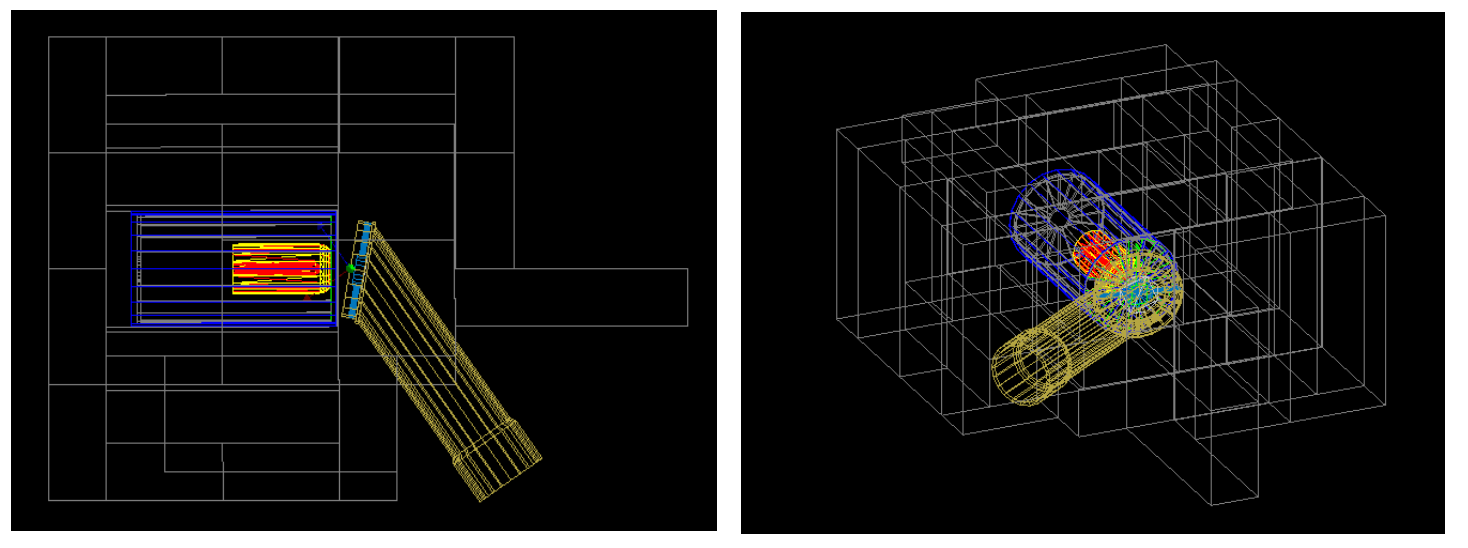
\includegraphics[width=\linewidth]{figures/shieldingSimulation.png}
\label{fig: simulatedSetup}
\caption{Simulation of the experimental setup at CASPAR, including the target chamber (in gold), water cooling (in light blue), HPGe detector (in dark blue), and lead bricks for shielding (in gray). Both pictures are of the same experimental setup from different angles to convey the layout. Simulating this setup is necessary to determine the total efficiency of the experimental setup. In this determination, a single-line $\gamma$ source is placed at the target location and its decays simulated for a variety of energies, allowing a determination of the total efficiency at each.}
\end{figure}


\begin{figure}
\centering
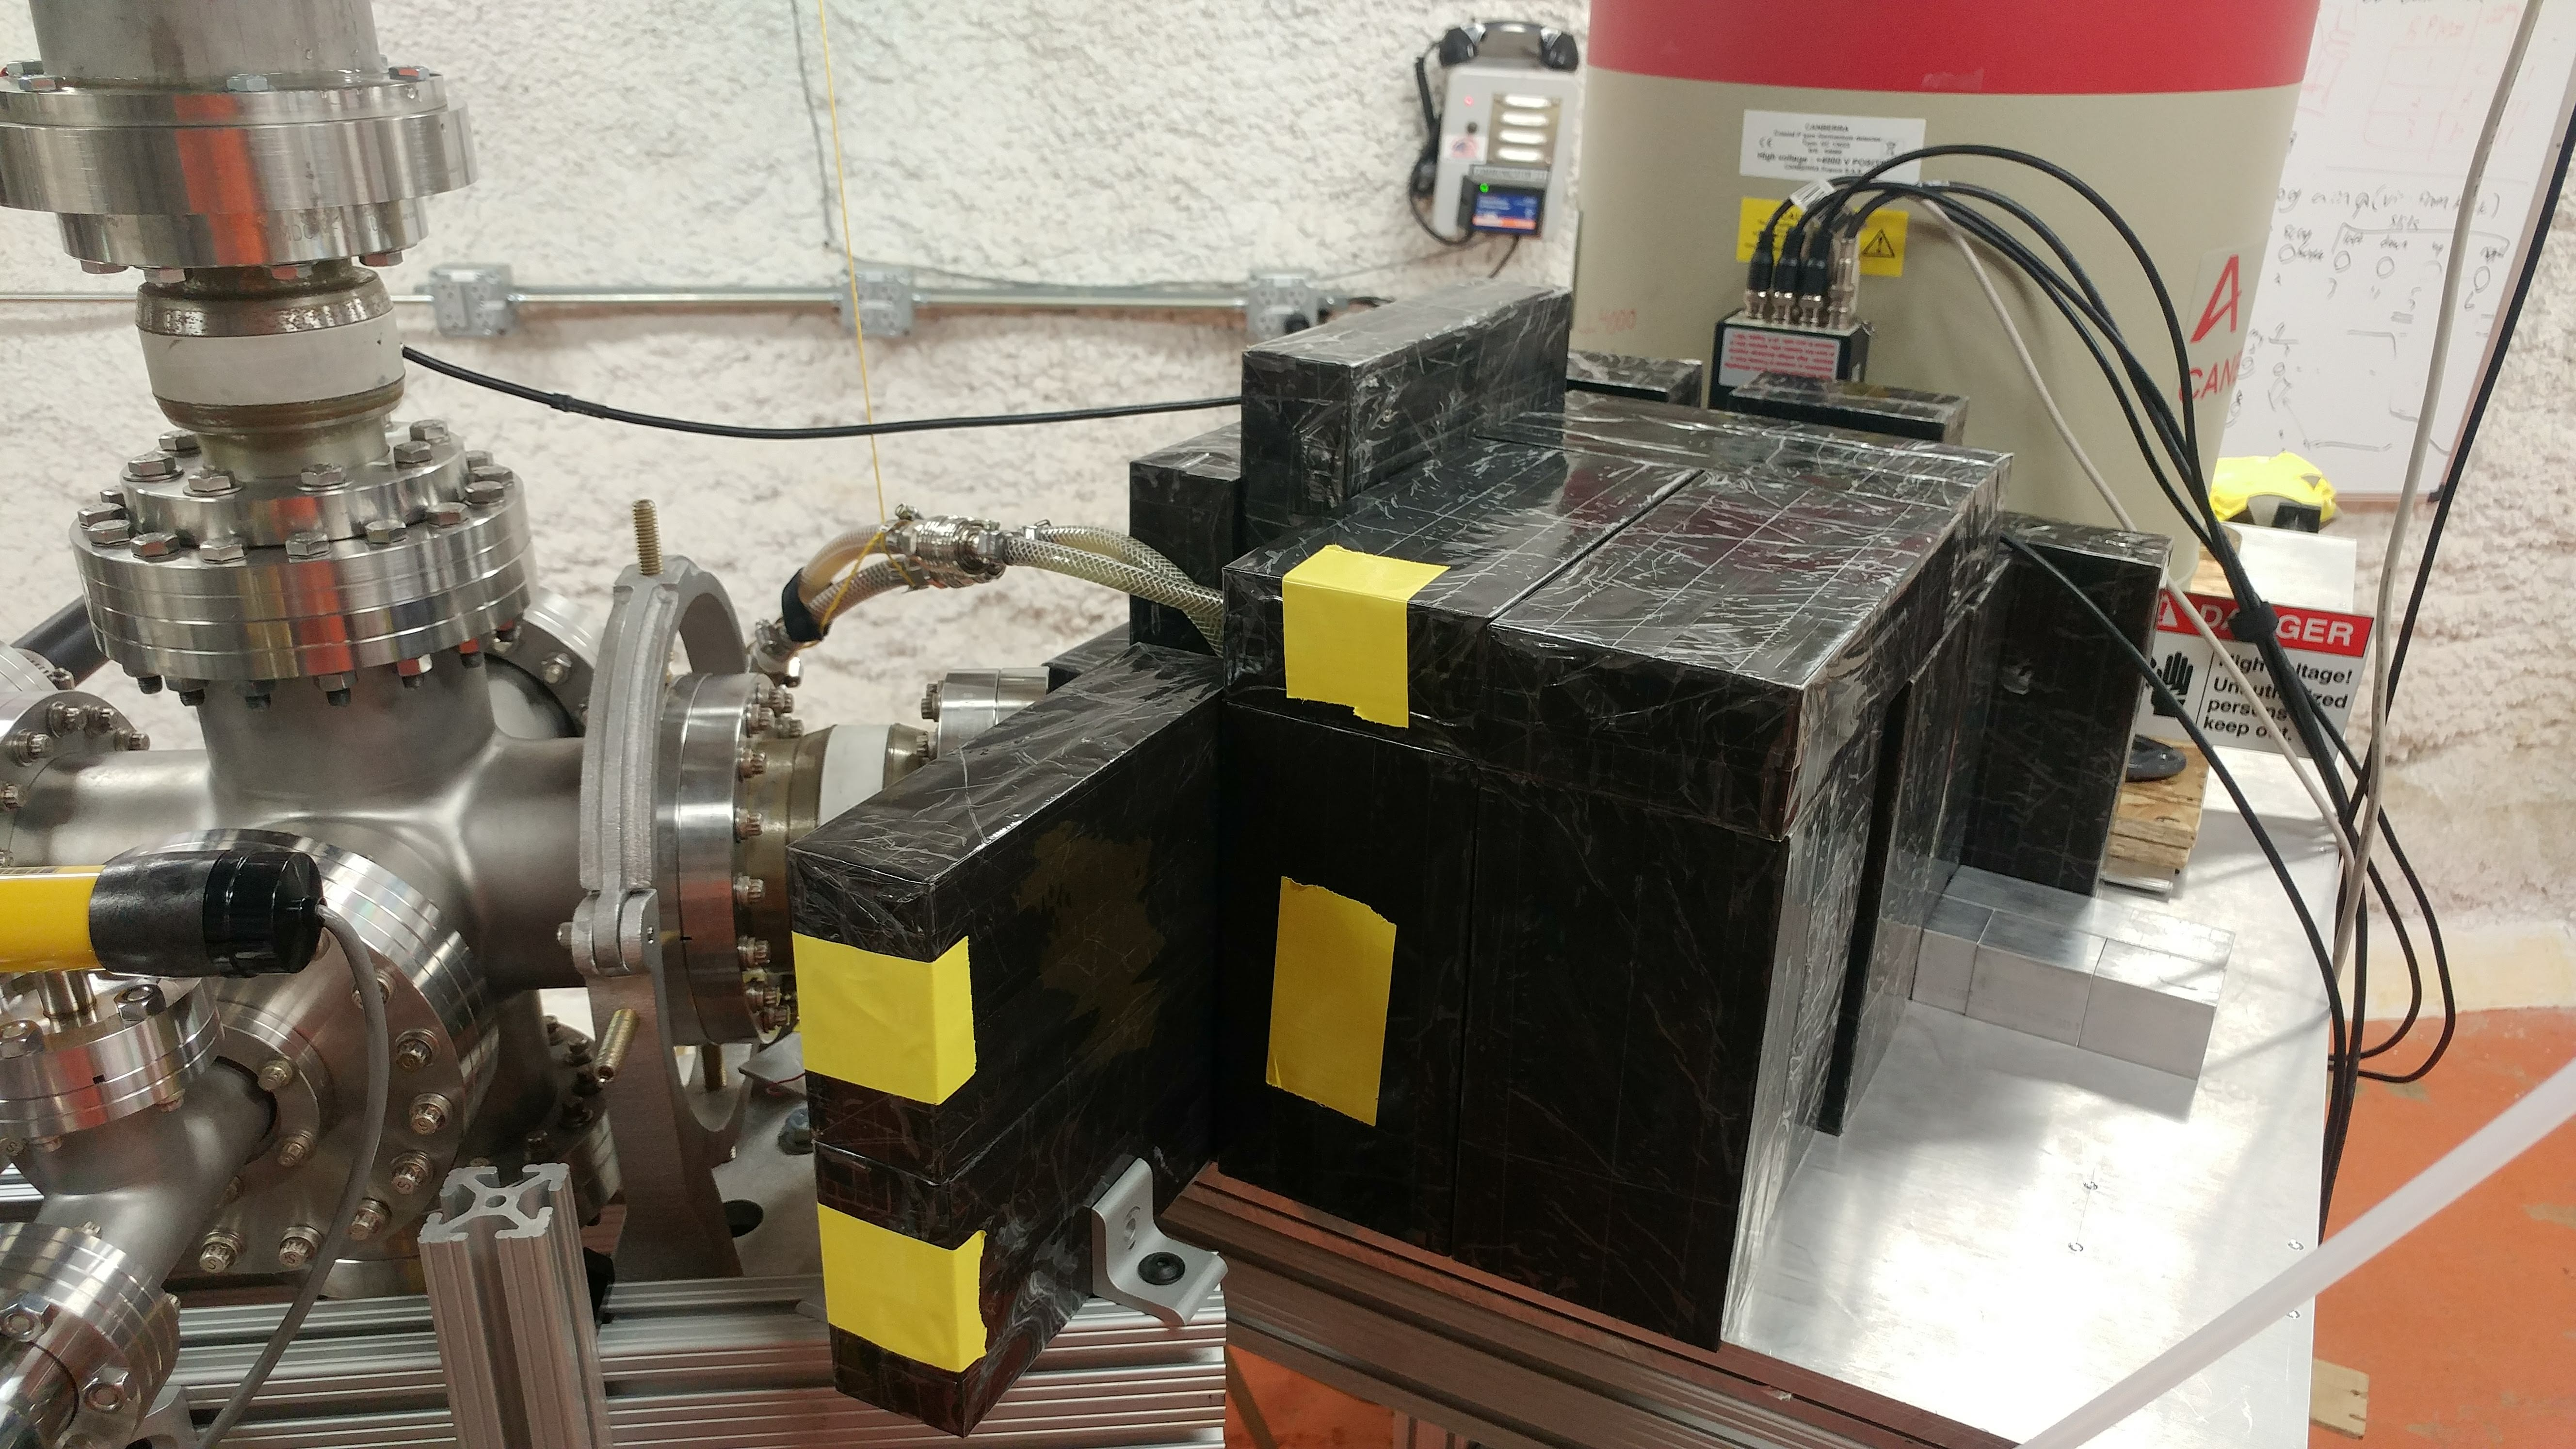
\includegraphics[width=0.8\linewidth]{figures/shieldingPicture.jpg}
\label{fig: actualSetup}
\caption{A picture of the experimental setup at CASPAR, showing the lead shielding around the detector and target chamber. This figure is provided for comparison to the simulated setup to prove its accuracy. }
\end{figure} 

To extend $\eta^{tot}$ to the whole range of energies relevant to the experiments, the experimental setup (including the target chamber, water cooling, and shielding) was built and simulated in Geant4 \cite{Agostinelli2003}, an example of the simulation for the CASPAR setup is shown in Fig.\ \ref{fig: simulatedSetup} where the actual setup is given in Fig.\ \ref{fig: actualSetup} for comparison. Then, a single-emission source was placed at the target location and simulated 10,000,000 decays, recording the deposited energy inside the detector. The energy of the source was changed and simulated at energies of 662, 1300, 2000, 3000, 4000, 6000, 7000, 8000, and 10000 keV to cover the entire range of $\gamma$ ray energies present in the $^{14}$N$\left( p,\gamma \right) ^{15}$O reaction. For each of the different decay energies, the spectrum of recorded events in the detector was analyzed in the exact same way as the actual $^{137}$Cs data to produce the total efficiency at each energy. This simulated data was used in conjunction with the measured $^{137}$Cs total efficiency data point to determine an accurate curve of the total efficiency across all experimentally relevant energies, shown in Fig.\ \ref{fig: totalEfficiency}.

\begin{figure}
\centering
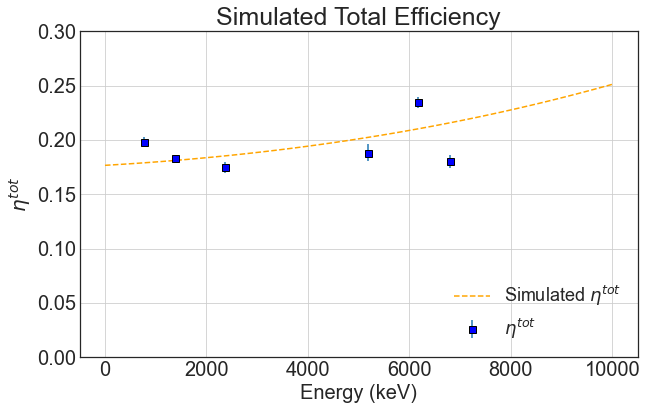
\includegraphics[width=\linewidth]{figures/totalEfficiency.png}
\label{fig: totalEfficiency}
\caption{The total efficiency of the HPGe in the CASPAR setup across all relevant energies. The points from the Geant4 simulation are taken raw without scaling, showing the efficacy of this technique and accuracy of the simulation.  }
\end{figure}



\subsection{Full energy peak efficiency}

The full energy peak (FEP) efficiency, on the other hand, is the probability that the full energy of a given photon will be recorded within the detector. Mathematically, this is

\begin{equation}
\eta^{FEP} = \dfrac{n(E)}{R(E)}
\end{equation}

\noindent where $n(E)$ is the count rate in the measured peak at an energy, $E$, where $R(E)$ is the rate at which photons of energy $E$ are emitted from the source \cite{DebertinHelmerBook}. From this point, if not specified, efficiency as a term is used to denote the FEP efficiency whereas the total efficiency will always be named explicitly. 

Determining the efficiency for a given setup is necessary for each geometry since, like the total efficiency, it is related to the specific source-detector geometry; it is not an intrinsic property of a given detector. In this campaign of experiments, the efficiency was determined each time with a combination of radioactive sources, like $^{137}$Cs, $^{60}$Co, and $^{152}$Eu, and well-known nuclear resonances, like $^{14}$N$\left( p,\gamma \right) ^{15}$O at $E_{p}$ = 278 keV and the $^{27}$Al($p, \gamma$)$^{28}$Si resonance at $E_{p}$ = 992 keV. These reactions were chosen because, much like the energy calibration, these extend the detector's measured efficiency to a much higher energy range (up to 10.7 MeV) compared to radioactive sources. 

From radioactive sources, the detector's efficiency at a given $\gamma$ ray energy, $\eta(E_{\gamma})$, can be determined with

\begin{equation}
\eta (E_{\gamma}) = \dfrac{N_{\gamma}}{A(t) B_{\gamma} t_{live} C_{i}},
\end{equation}

\noindent where $N_{\gamma}$ is the measured number of counts in the full energy peak, $A(t)$ is the source's activity at the time of the measurement, $B_{gamma}$ is the branching ratio for the specific decay, $t_{live}$ is the live time of the measurement, and $C_{i}$ are the correction factors, if necessary. For nuclear resonances, on the other hand, $\eta (E_{gamma})$ is 

\begin{equation}
\eta (E_{\gamma}) = \dfrac{N_{\gamma}}{q B_{\gamma} R C_{i}},
\end{equation}

\noindent where $q$ is the collected charge and

\begin{equation}
R = \dfrac{\lambda_{r}^{2}}{\pi} \dfrac{\omega \gamma}{\epsilon_{sp}} \dfrac{M + m}{M} \tan^{-1} \left( \dfrac{\Delta E}{\Gamma}  \right)
\label{eqn: resonanceFactor}
\end{equation}

\noindent with $\lambda_{r}$ is the proton's de Broglie wavelength at the resonance energy, $\omega \gamma$ is the resonance strength (as defined in Chapter \ref{chap: introduction}), $\epsilon_{sp}$ is the stopping power of the target at the resonance energy, $M$ is the target atomic mass, $m$ is the projectile atomic mass, $\Delta E$ is the thickness of the target, and $\Gamma$ is the resonance width. 

For this determination, the branching ratios for the 278 keV resonance in $^{14}$N$\left( p,\gamma \right) ^{15}$O were taken from Daigle \textit{et al.} \cite{Daigle2016} where for the 992 keV resonance in $^{27}$Al($p, \gamma$)$^{28}$Si they were obtained from Antilla \textit{et al.} \cite{Antilla1977} and those from the 406 keV resonance in $^{27}$Al($p, \gamma$)$^{28}$Si are taken from Powell \textit{et al.} \cite{Powell1998}. The efficiencies were then fit with 

\begin{equation}
\eta = \exp \left(  \sum_{i=0}^{3} a_{i} ( \ln (E_{\gamma}))^{2}    \right),
\end{equation}

\noindent where the $a_{i}$ are fit coefficients and $E_{\gamma}$ is the $\gamma$-ray energy and the independent variable in the fit. An example of this determination for the CASPAR setup in both the close and far geometries can be seen in Fig. \ref{fig: efficiency}. In both calculations, only statistical errors were included in the fit and the highest energy point was excluded due to summing effects, which will be discussed in more detail in the next section. This can be clearly seen as the highest energy point at close distance (1.1 cm from target) is off by an inordinately large factor. For a reference, measurements were also taken at 25.24 cm away from the target chamber, making the summing effects negligible. In this case, the summing effects provide very little impact (if any) on the highest energy point, which was still excluded from this fit. However, for the far distance it follows the trend of the other data nearly perfectly.


\begin{figure}
\centering
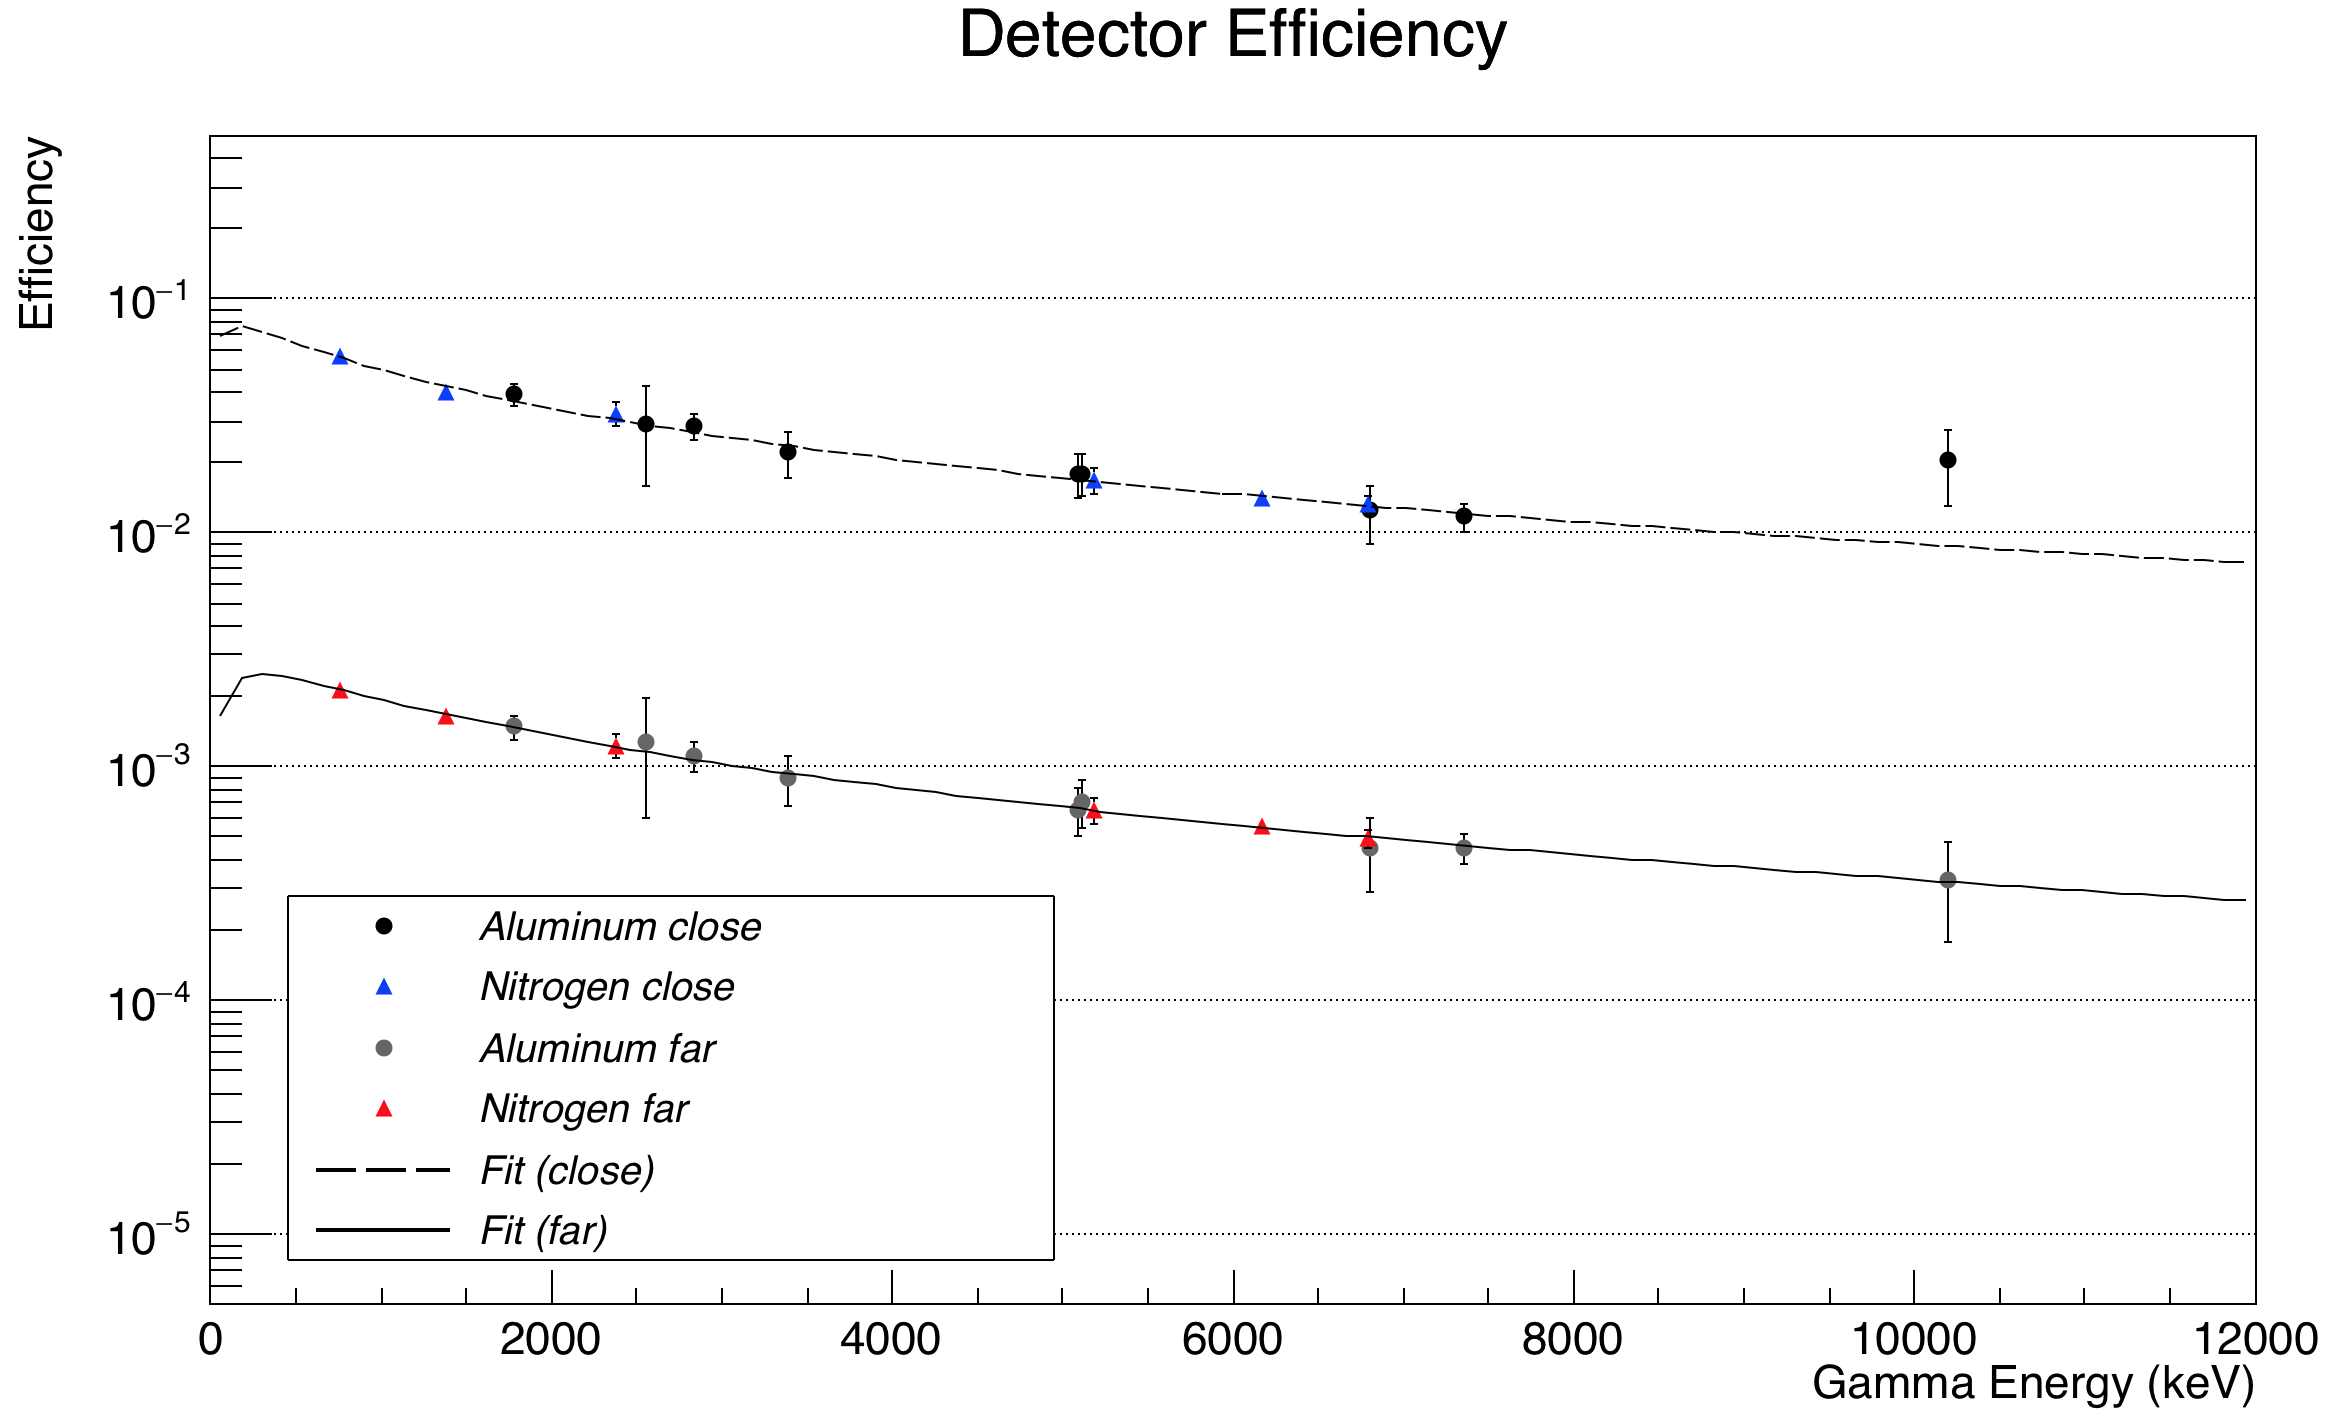
\includegraphics[width=\linewidth]{figures/efficiencyComplete.png}
\label{fig: efficiency}
\caption{Detector efficiency as a function of $\gamma$-ray energy for the measurement at CASPAR in both close and far geometries. The highest energy point in the close geometry was excluded from the fit because it suffers from summing-in effects artificially inflating the count rate of this measured peak (see text for details). At the far distance between the detector and the target, summing effects are negligible. This can be seen as the highest-energy data point now lies perfectly with the fit from the other data.  }
\end{figure}



\section{Summing corrections}
\label{sec: summing}

Summing corrections need to be applied to data due to data-recording phenomena manifesting in measured spectra. There are two different ways in which the recorded data can be affected, the so-called summing-in and summing-out effects, and these are more pronounced when measurements happen with the detector and source in close proximity or with simple reaction product decay structures, as in the case in the $^{14}$N$\left( p,\gamma \right) ^{15}$O reaction.


\begin{figure}
\centering
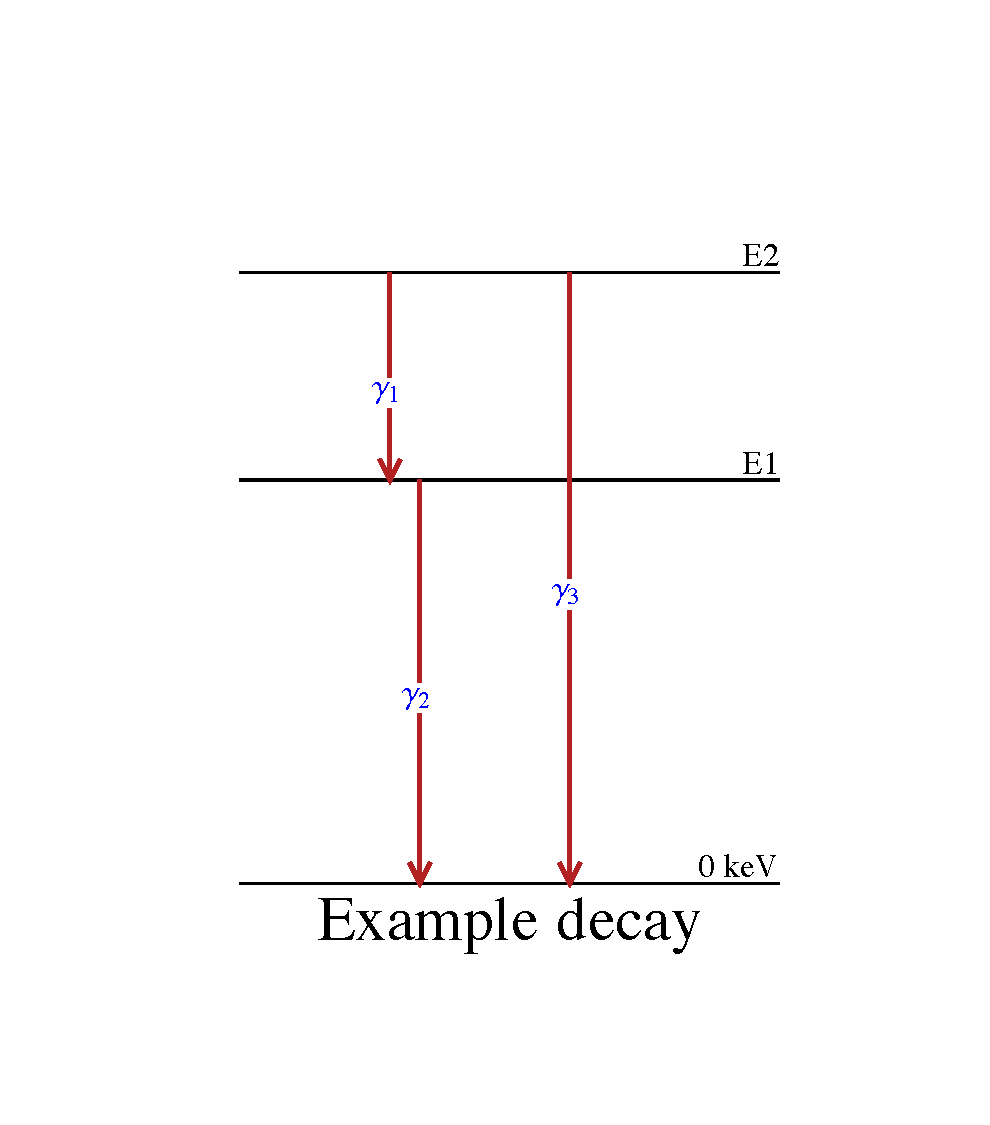
\includegraphics[width=0.7\linewidth]{figures/simpleScheme.pdf}
\label{fig: simpleDecay}
\caption{Example cascade nuclear decay for demonstrating summing effects (see text for details). }
\end{figure}

For a simple nuclear decay, like that in Fig. \ref{fig: simpleDecay}, summing manifests in a measured spectrum in two different ways. If any portion of the energy from $\gamma_{1}$ is deposited in the detector simultaneous with $\gamma_{2}$, the the resultant recorded event will have an energy higher than either individual $\gamma$-ray and, therefore, will appear at a different energy in the spectrum. Consequently, $\gamma_{2}$'s count rate will be artificially lowered. By the same logic, the count rate for $\gamma_{1}$ will also be artificially dropped. This loss of counts in the peaks recorded at energies $E_{1}$ and $E_{2}$ is known as the summing-out effect. As an extension of this thought experiment, if the full energy of both $\gamma_{1}$ and $\gamma_{2}$ is deposited in the detector at the same time the resulting measured energy will match $E_{3}$, artificially inflating the count rate of that peak. This increase is called the summing-in effect.

To correct for these effects, the probability of measuring a different energy than expected must be taken into account. For a situation where there is no summing, the rate of $\gamma$ rays is simply the yield

\begin{equation}
Y_{i} = R B_{i} \eta_{i},
\end{equation}

\noindent where $R$ is the normalization from Equation \ref{eqn: resonanceFactor}, $B$ is the branching ratio, and $\eta$ is the FEP efficiency. However, when summing-out occurs, the yield is artificially dropped by the factor $R B \eta_{1} \eta^{tot}_{2}$, which is the probability of counting the full energy of $\gamma_{1}$ along with any part of $\gamma_{2}$. Mathematically, this observed yield for both $\gamma_{1}$ and $\gamma_{2}$ is

\begin{align}
Y_{1} &= R B_{1} \eta_{1} - R B_{1} \eta_{1} \eta^{tot}_{2} \\
        &= R B_{1} \eta_{1} \left( 1 - \eta^{tot}_{2} \right) \\
Y_{2} &= R B_{2} \eta_{2} \left( 1 - \eta^{tot}_{1} \right).
\end{align}

\noindent Then, in order to correct for this, the ratio of the true emitted $\gamma$'s to the observed rate for $\gamma_{1}$ is

\begin{equation}
\dfrac{Y_{1}}{Y^{obs}_{1}} = \dfrac{1}{1 - \eta^{tot}_{2}} = C_{1},
\end{equation}

\noindent where the $C_{i}$ is the correction factor. The same relation holds for $\gamma_{2}$. This makes clear why the total efficiency is so important: without it, summing-out is not an effect which can be corrected. For $\gamma_{3}$, however, the situation requires the total energy deposition of $\gamma_{1}$ and $\gamma_{2}$ at the same time, so correcting for summing-in requires the FEP efficiency. This is

\begin{equation}
Y_{3} = R B_{3} \eta_{3} + R B_{1} \eta_{1} \eta_{2}
\end{equation} 

\noindent where the second term includes $B_{1}$ because the decay chain has to start with $\gamma_{1}$. By the same token, the correction factor for summing-in is

\begin{equation}
C_{3} = \dfrac{Y_{3}}{Y_{3}^{obs}} = \dfrac{1}{1 + \left( \dfrac{B_{1} \eta_{1} \eta_{2}} {B_{3} \eta_{3}}  \right)}.
\end{equation}


With a more complicated nuclear level scheme, the summing corrections become more difficult to apply accurately. A more detailed treatment of the necessary methods can be found in \cite{DebertinHelmerBook}. This is primarily due to more complicated feeding and the presence of multiple decays from a given level. In general, the correction is for the $i$th level is

\begin{align}
C_{i} &= 1 + C_{i}^{in} - C_{i}^{out} \\
C_{i}^{in} &= \sum_{m,n} \dfrac{B_{m} p_{n} \eta_{m} \eta_{n}}{B_{i} \eta_{i}} \\
C_{i}^{out} &= \sum_{j,k} p_{k} \eta_{k}^{tot} + \dfrac{B_{j} p_{i} \eta_{j}^{tot}}{B_{i}}
\end{align}

\noindent where the $p_{i}$ are the probability of feeding. Fortunately, for the $^{15}$O nucleus, all intermediate decays have a branching ratio of 100\%, as can be seen in \ref{fig: summingOxygen}. The summing out corrections in each case can then be

\begin{equation}
C_{i}^{out} = 1 - \eta^{tot}_{j},
\end{equation}

\noindent where the $i$ and $j$ denote the $\gamma$ rays feeding into and decaying from the state, respectively (like $\gamma_{1}$ and $\gamma_{6}$ for example). For this measurement, the summing-out effect for every transition except the ground state is relatively small, falling in the range of 3.6 - 5.2 \% for all of the relevant $\gamma$'s.

Conversely, only the R/DC$\rightarrow$GS transition needs to be corrected for summing-in effects as the total energy of the other decay branches matches the energy of $\gamma_{7}$, and, as such, should be a larger effect since the true branch to the ground state is $\sim 4$\%. The observed yield of $\gamma_{7}$ in this case will be

\begin{equation}
Y_{7} = R B_{7} \eta_{7} + R B_{1} \eta_{1} \eta_{6} +  R B_{2} \eta_{2} \eta_{5} + R B_{3} \eta_{3} \eta_{4} .
\end{equation}

\noindent From this, then, the correction factor for the ground state transition will necessarily be

\begin{equation}
C_{7}^{in} = 1 + \dfrac{B_{1} \eta_{1} \eta_{6} + B_{2} \eta_{2} \eta_{5} + B_{3} \eta_{3} \eta_{4} }{B_{7} \eta_{7}}.
\end{equation}

\noindent In this measurement, this correction is quite large - on the order of $\sim$\textbf{PERCENT}\%. 


\begin{figure}
\hspace{-2cm}
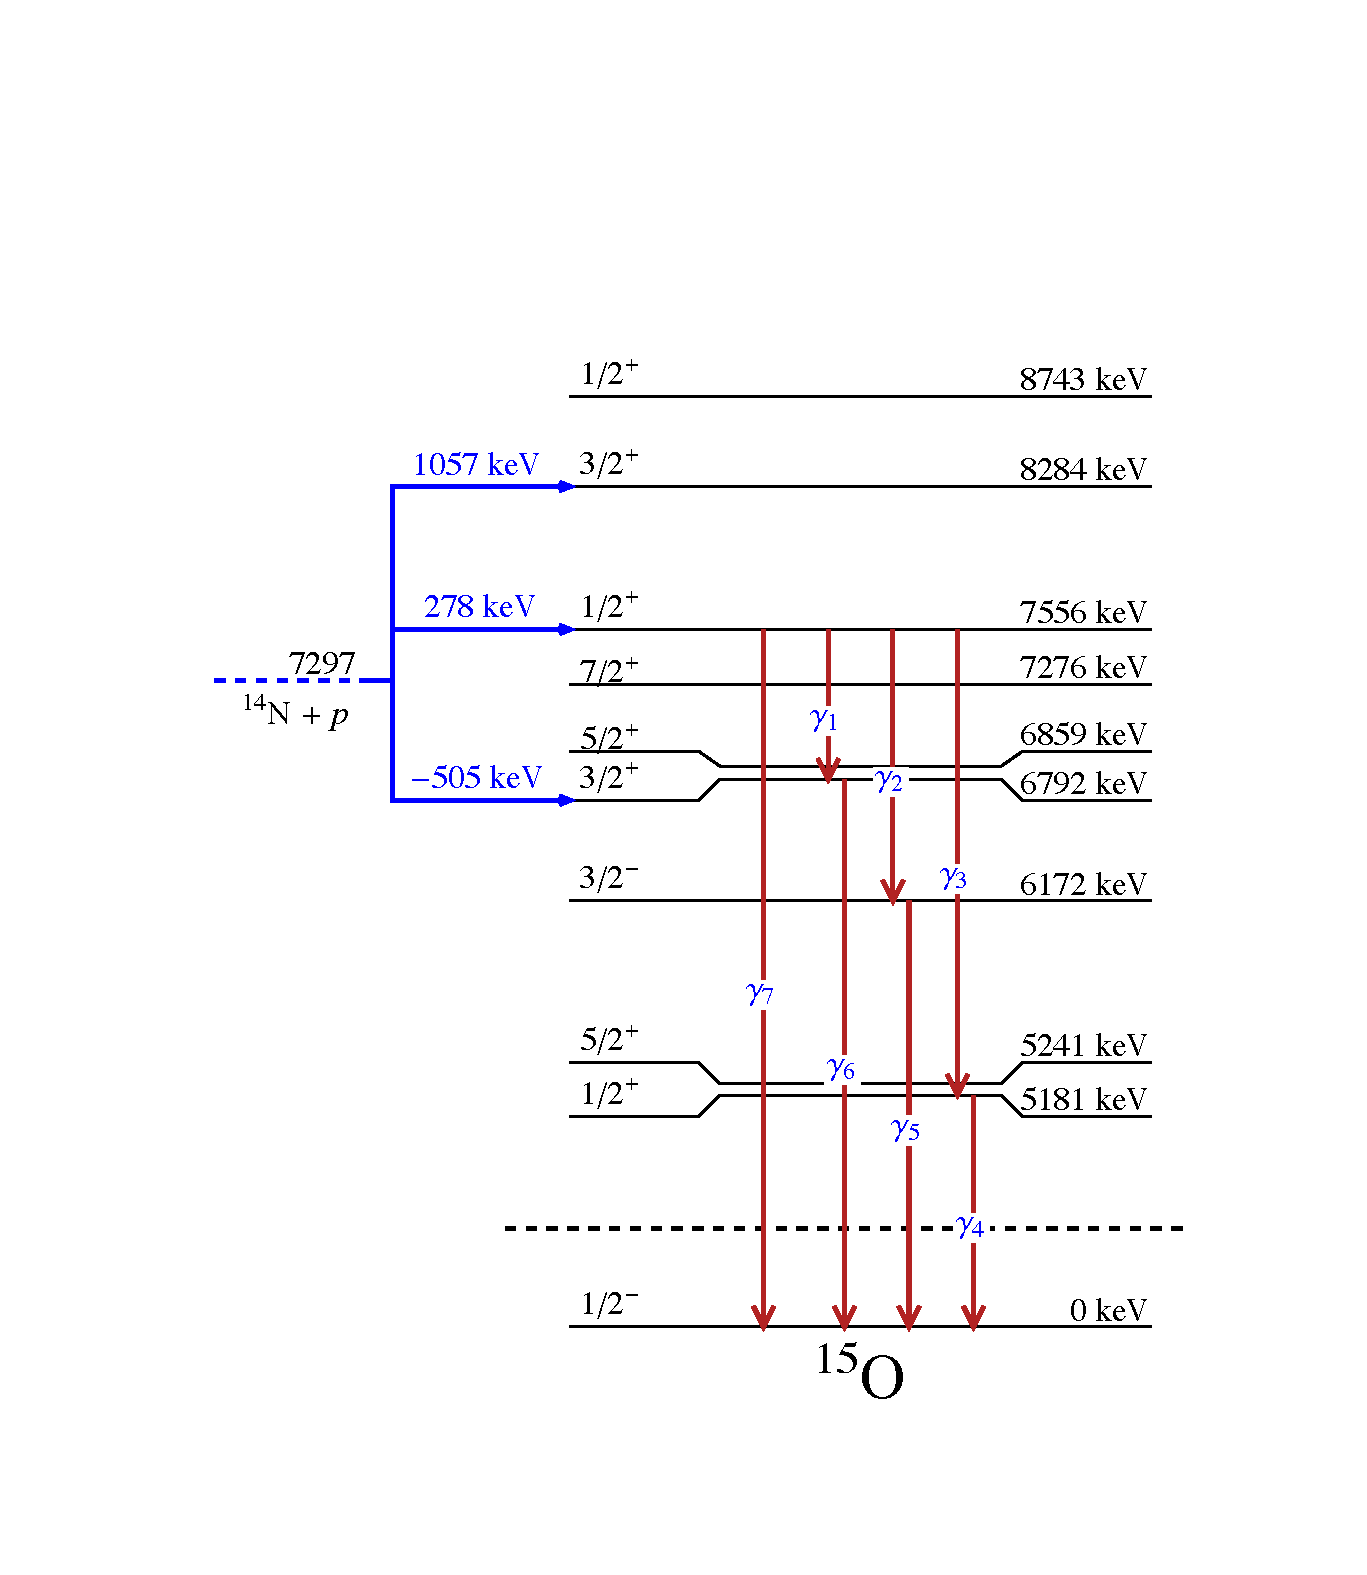
\includegraphics[width=1.0\linewidth]{figures/summingOxygenDecays.pdf}
\label{fig: summingOxygen}
\caption{All decays from the 278 keV proton resonance in the $^{14}$N$\left( p,\gamma \right) ^{15}$O reaction. Other than the resonance level, all decays are sequential, with the levels having only one decay directly to ground state. Of note, this then means that the total energy for each decay sequence matches the direct transition, $\gamma_{7}$, so it must be corrected for summing-in effects from all the other branches. }
\end{figure}




\section{Target characterization}
\label{sec: target}

\section{Cross-section determination}
\label{sec: cross-section}





% % uncomment the following lines,
% if using chapter-wise bibliography
%
% \bibliographystyle{ndnatbib}
% \bibliography{example}
